We discussed the life cycle of a C++ program in Chapter 5, Compiling C++ Sources with CMake. It consists of five main stages – writing, compiling, linking, loading, and execution. After correctly compiling all the sources, we need to put them together into an executable. Object files produced in a compilation can't be executed by a processor directly. But why?

To answer this, let's take a look at how a compiler structures an object file in the popular ELF format (used by Unix-like systems and many others):

\begin{center}
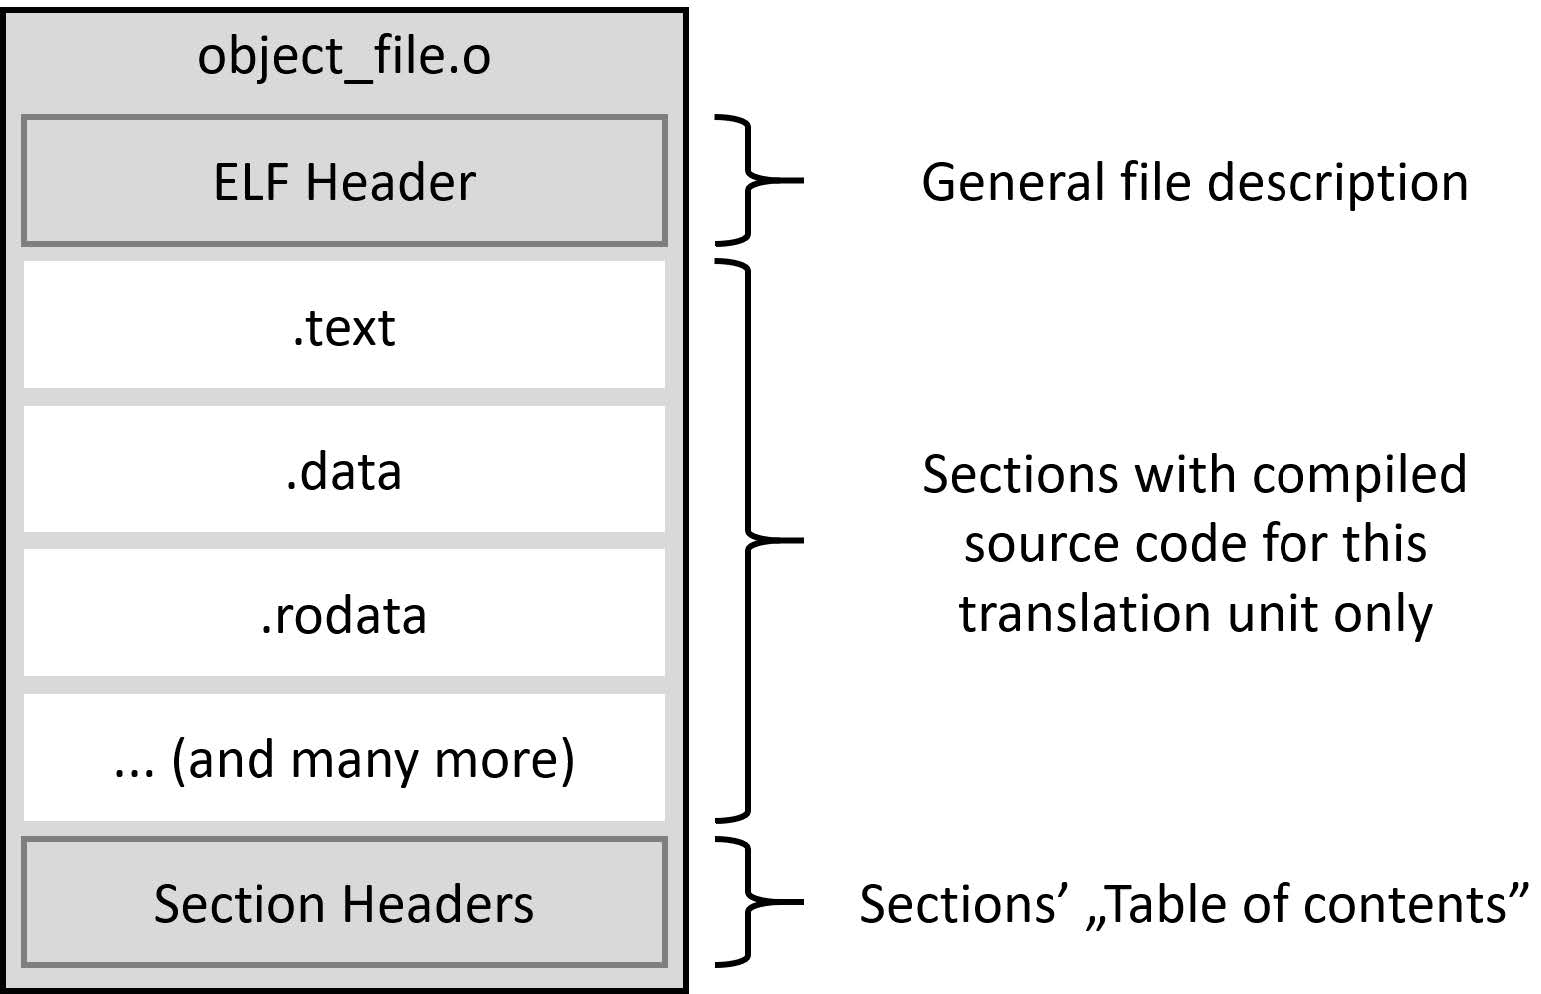
\includegraphics[width=0.8\textwidth]{content/2/chapter6/images/1.jpg}\\
Figure 6.1 – The structure of an object file
\end{center}

The compiler will prepare an object file for every unit of translation (for every .cpp file). These files will be used to build an in-memory image of our program. Object files contain the following elements:

\begin{itemize}
\item 
An ELF header identifying the target operating system, ELF file type, target instruction set architecture, and information on the position and size of two header tables found in ELF files – the program headers table (not present in object files) and the section headers table.

\item 
Sections containing information grouped by type (described next).

\item 
A section headers table, containing information about the name, the type, flags, the destination address in memory, the offset in the file, and other miscellaneous information. It is used to understand what sections are in this file and where they are, just like a table of contents.
\end{itemize}

As the compiler processes your source code, it groups the collected information into a few separate bins, which will be put in their own separate section. Some of them are as follows:

\begin{itemize}
\item 
.text section: Machine code, with all the instructions to be executed by the processor

\item 
.data section: All values of the initialized global and static objects (variables)

\item 
.bss section: All values of the uninitialized global and static objects (variables), which will be initialized to zero on program start

\item 
.rodata section: All values of the constants (read-only data)

\item 
.strtab section: A string table containing all constant strings such as Hello World that we put in our basic hello.cpp example

\item 
.shstrtab section: A string table containing the names of all the sections
\end{itemize}

These groups very closely resemble the final version of the executable, which will be put in the RAM to run our application. However, we can't just load this file to memory as it is. This is because every object file has its own set of sections. If we were to just concatenate them together, we'd run into all sorts of issues. We'd be wasting a lot of space and time, as we'd need many more pages of RAM. Instructions and data would be much harder to copy to a CPU cache. An entire system would have to be much more complex and would waste precious cycles jumping around many (possibly tens of thousands) of .text, .data, and other sections during runtime.

So, what we'll do instead is take each section of the object file and put it together with the same type of section from all other object files. This process is called relocation (that's why the ELF file type is Relocatable for object files). Apart from just bringing appropriate sections together, it has to update internal associations in the file – that is, addresses of variables, functions, symbol table indexes, or string table indexes. All of these values are local to the object file, and their numbering starts from zero. When we bundle files together, we need to offset these values so that they are pointing at the correct addresses in the combined file.

Figure 6.2 shows relocation in action – the .text section is relocated, .data is being built from all linked files, and .rodata and .strtab will follow (for simplicity, the figure doesn't contain headers):

\begin{center}
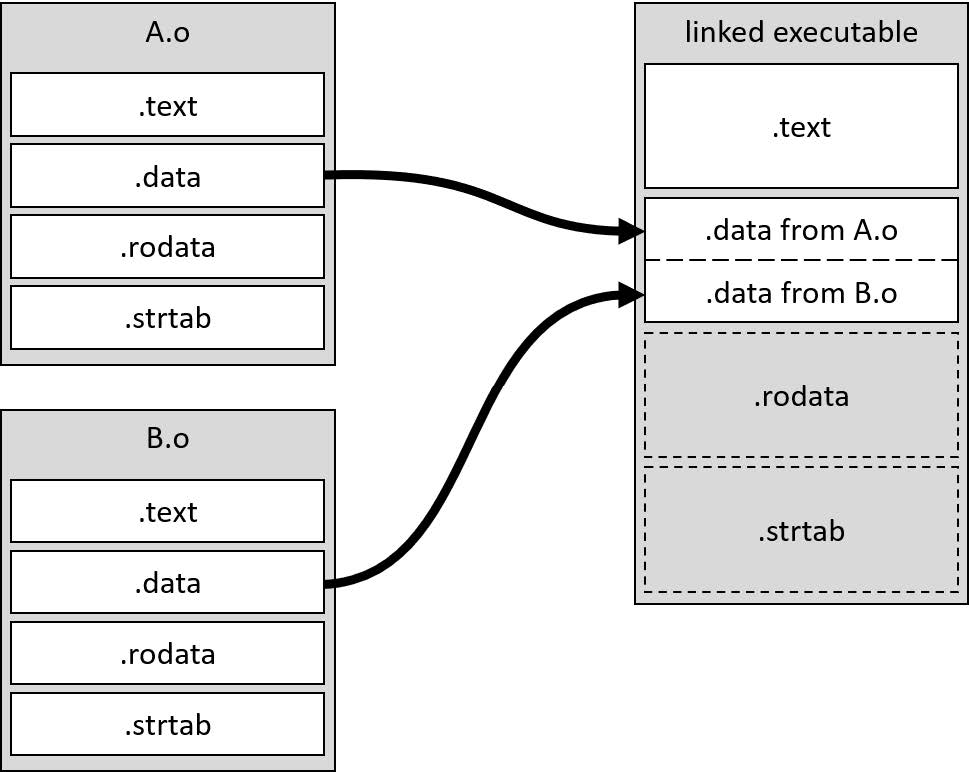
\includegraphics[width=0.8\textwidth]{content/2/chapter6/images/2.jpg}\\
Figure 6.2 – The relocation of the .data section
\end{center}

Secondly, a linker needs to resolve references. Whenever a piece of code from one translation unit references a symbol defined in another (such as through including its header or by using the extern keyword), the compiler reads the declaration and trusts that the definition is somewhere out there and will be provided at a later time. A linker is responsible for collecting such unresolved references to external symbols, finding and filling the addresses at which they reside after merging into the executable. Figure 6.3 shows a simple example of reference resolution:

\begin{center}
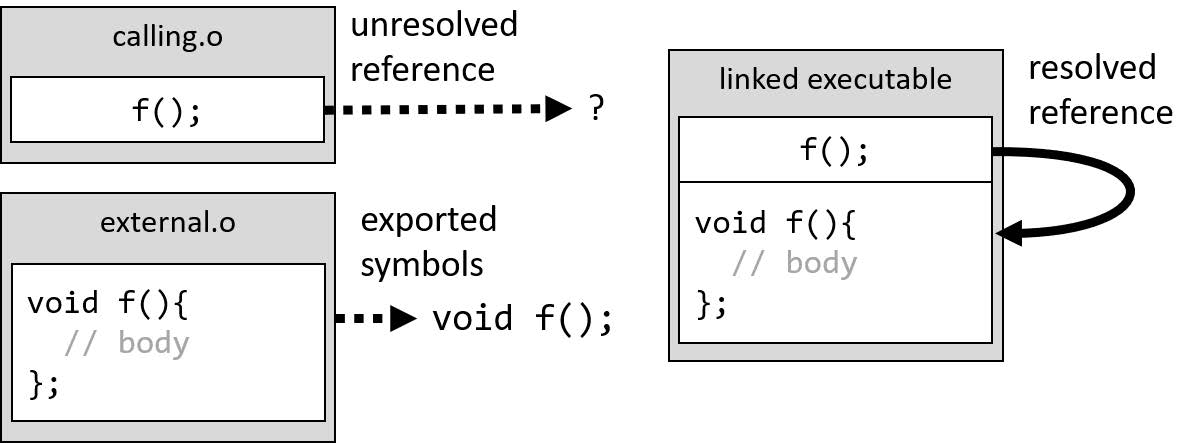
\includegraphics[width=0.8\textwidth]{content/2/chapter6/images/3.jpg}\\
Figure 6.3 – A reference resolution
\end{center}

This part of the linking can be a source of problems if a programmer is unaware of how it works. We may end up with unresolved references that won't find their external symbols, or the opposite – we provided too many definitions and the linker doesn't know which one to pick.

The final executable file looks very similar to the object file; it contains relocated sections with resolved references, a section headers table, and of course, the ELF Header describing the whole file. The main difference is the presence of the Program Header (as pictured in Figure 6.4).

\begin{center}
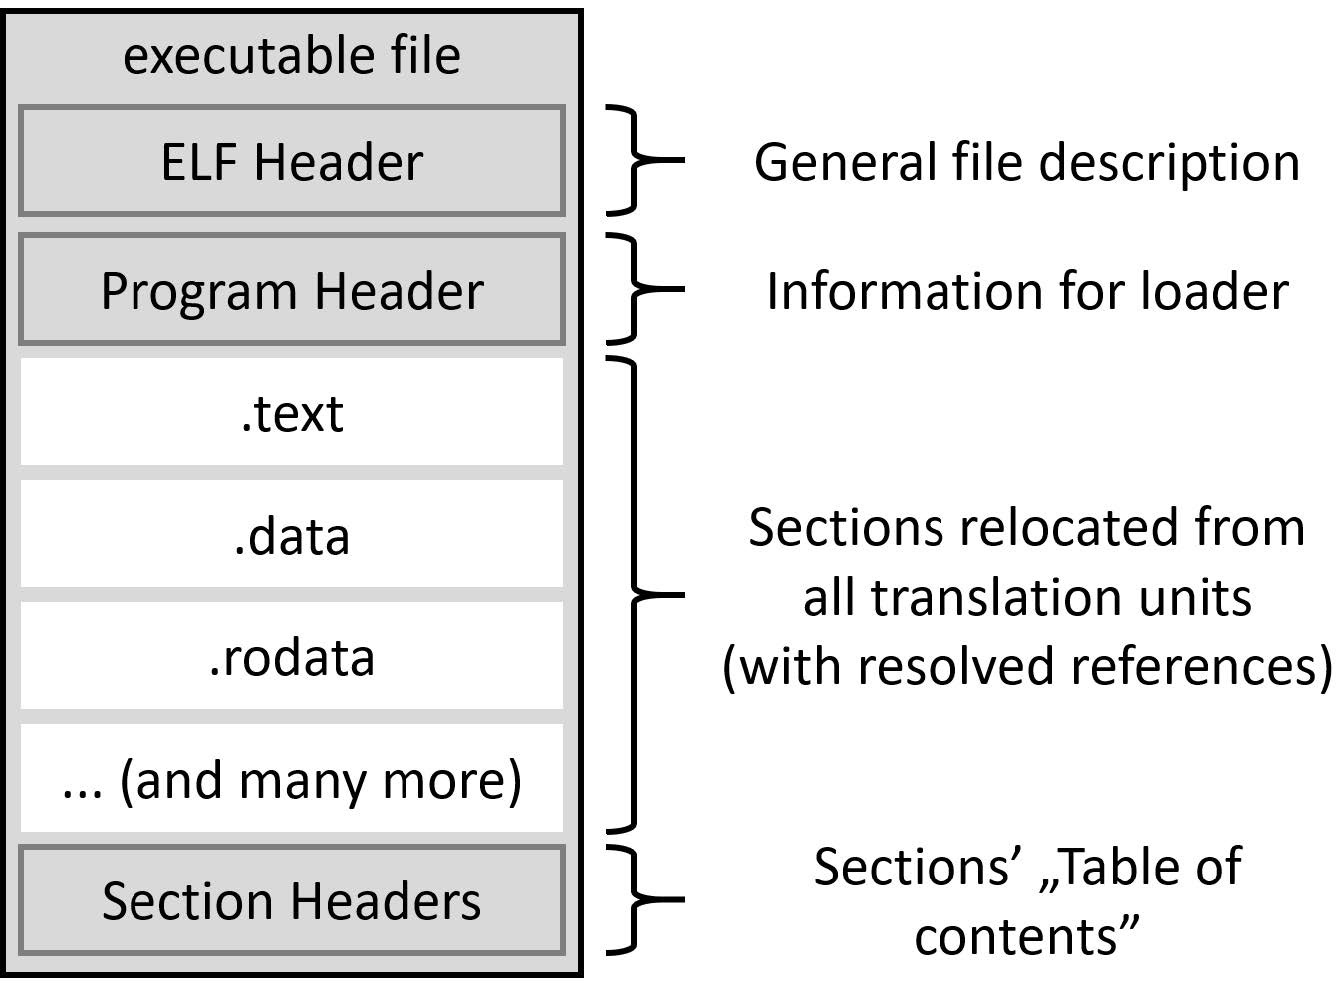
\includegraphics[width=0.8\textwidth]{content/2/chapter6/images/4.jpg}\\
Figure 6.4 – The structure of the executable file in ELF
\end{center}

The Program Header is placed right after the ELF Header. A system loader will read this header to create a process image. The header contains some general information and a description of the memory layout. Each entry in the layout represents one fragment of memory called a segment. Entries specify which sections will be read, in what order, to which addresses in the virtual memory, what their flags are (read, write, or execute), and a few other useful details.

Object files may also be bundled in a library, which is an intermediate product that can be used in a final executable or another library. In the next section, we'll discuss three types of libraries.



